\renewcommand{\theequation}{\theenumi}
\begin{enumerate}[label=\arabic*.,ref=\thesubsection.\theenumi]
\item Find the equation of a circle which passes through the points $\myvec{2\\-1}$, $\myvec{1\\-2}$ and cuts orthogonally the circle
\begin{align}
\vec{x}^T\vec{x}+\myvec{-2 & 3}\vec{x}-5 = 0
\end{align}
\numberwithin{equation}{enumi}
\item Find the equation of a circle which cuts orthogonally the three circles
\begin{align}
\vec{x}^T\vec{x}+\myvec{4 & -5}\vec{x}+6 = 0
\\
\vec{x}^T\vec{x}+\myvec{5 & -6}\vec{x}+7 = 0
\\
\vec{x}^T\vec{x}-\myvec{1 & 1}\vec{x}-1 = 0
\end{align}
\item Find the equation of a circle which cuts orthogonally the two circles
\begin{align}
\vec{x}^T\vec{x}-\myvec{2 & 2}\vec{x}+1 = 0
\\
\vec{x}^T\vec{x}+\myvec{-3 & 6}\vec{x}-2 = 0
\end{align}
and passes through the point $\myvec{-3\\2}$.
\item Write down the equations of the radical axes of the following pairs of circles:
\begin{enumerate}
\item
%
\begin{align}
\vec{x}^T\vec{x}-\myvec{4 & -5}\vec{x}-2 = 0
\\
\vec{x}^T\vec{x}-\myvec{5 & -6}\vec{x} = 0
\end{align}
%
\item
\begin{align}
%
\vec{x}^T\vec{x}+\myvec{3 & -2}\vec{x}+1 = 0
\\
\vec{x}^T\vec{x}-\myvec{3 & -5}\vec{x}+2 = 0
\end{align}
%
\item
\begin{align}
%
\vec{x}^T\vec{x}+2g\myvec{1 & 0}\vec{x}+c = 0
\\
\vec{x}^T\vec{x}+2f\myvec{0 & 1}\vec{x}+c = 0
\end{align}
%
\end{enumerate}
\solution

Given, two circles with equations,
\begin{align}
S=\vec{x}^{T}\vec{x}-\myvec{4 & -5}\vec{x}-2=&0\label{rams/4/4/4/a/eq:1}\\
S'=\vec{x}^{T}\vec{x}-\myvec{5 & -6}\vec{x}=&0\label{rams/4/4/4/a/eq:2}
\end{align}
We know, the radical axis for the pair of circles, $S=0, S'=0$ is given by $L=S-S'=0$.\\
Using \eqref{rams/4/4/4/a/eq:1}, \eqref{rams/4/4/4/a/eq:2}, the required equation is
\begin{align}
\brak{\vec{x}^{T}\vec{x}-\myvec{4 & -5}\vec{x}-2}-\brak{\vec{x}^{T}\vec{x}-\myvec{5 & -6}\vec{x}=0}=&0\\
\myvec{1 & -1}\vec{x}-2=&0
\end{align}
$\therefore L=\myvec{1 & -1}\vec{x}-2=0$ is the equation of the required radical axis.  See Fig.  \ref{rams/4/4/4/a/plot}
\begin{figure}[!h]
 \centering
 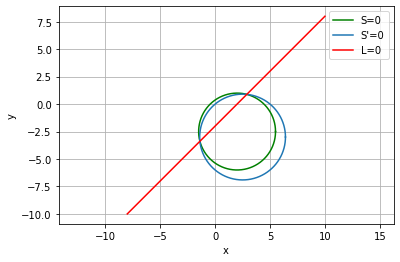
\includegraphics[width=\columnwidth]{solutions/4/4/4/a/figures/Assignment3.png}
 \caption{Pair of Circles and their radical axis}
 \label{rams/4/4/4/a/plot}
\end{figure}

\item Find the equation of a circle coaxal with
\begin{align}
\vec{x}^T\vec{x}-\myvec{2 & -3}\vec{x}-1 &= 0
\\
\vec{x}^T\vec{x}+\myvec{3 & -2}\vec{x}-1 &= 0
\end{align}
and passing through the point $\myvec{2\\1}$.
\item Find the coordinates of the point from which the tanges to the three circles
\begin{align}
\vec{x}^T\vec{x}-\myvec{4 & 4}\vec{x}+7 = 0
\\
\vec{x}^T\vec{x}+\myvec{4 & 0}\vec{x}+3 = 0
\\
\vec{x}^T\vec{x}+\myvec{0 & 2}\vec{x} = 0
\end{align}
are of equal length.
\item Find the limiting points of the circles
\begin{align}
\vec{x}^T\vec{x}+\myvec{0 & 2}\vec{x}-4 &= 0
\\
\vec{x}^T\vec{x}+\myvec{2 & 2}\vec{x}-10 &= 0
\end{align}
\item Prove that if a point moves so that the tangent from it to the circle
\begin{align}
\vec{x}^T\vec{x}+\myvec{4 & -5}\vec{x}+6 = 0
\end{align}
is double the length of the tangent to the circle
\begin{align}
\norm{\vec{x}} = 2,
\end{align}
its locus is the circle
\begin{align}
3\vec{x}^T\vec{x}-\myvec{4 & -5}\vec{x}-22 = 0
\end{align}
\item Prove that the locus of a point such that the lengths of the tangents from it to two given circles are in a constant ratio is a circle
coaxal with the given circles.
\item Find the equations of the two circles coaxal with
\begin{align}
\vec{x}^T\vec{x}-\myvec{8 & -10}\vec{x}+2 = 0
\\
\vec{x}^T\vec{x}-\myvec{3 & -5}\vec{x}-1 = 0
\end{align}
that touch the line
\begin{align}
\myvec{2 & 1}\vec{x}-3 = 0
\end{align}
\item Find the centre and radius of the circle which cuts orthogonally the three circles
\begin{align}
\vec{x}^T\vec{x}-\myvec{6 & 4}\vec{x}+12 = 0
\\
\vec{x}^T\vec{x}+2\myvec{1 & 1}\vec{x}+1 = 0
\\
\vec{x}^T\vec{x}+\myvec{4 & -2}\vec{x}+4 = 0
\end{align}
\item The line 
\begin{align}
\myvec{1 & 3}\vec{x}+2 = 0
\end{align}
is the radical axis of a family of coaxal circles of which one circle is
\begin{align}
\vec{x}^T\vec{x}+\myvec{2 & 5}\vec{x}-1 = 0.
\end{align}
Find the equation of the member of the family that passes through the point $\myvec{-3\\1}$.
\end{enumerate}
